\section{Prechodové a frekvenčné charakteristiky}
V tejto kapitole sú prezentované výsledky simulácií prechodových a frekvenčných charakteristík modelu synchrónneho generátora. Prechodové charakteristiky boli získané simuláciou modelu v Simulinku, kde ako referenčný signál napätia bol použitý skokový signál. Skoky boli realizované ako $2\%$ zmeny referenčného napätia, ktorého počiatočná hodota bola nastavená na $0.98$ pomerných jednotiek ($p.u.$), a teda prvý skok bol realizovaný na $1.00 p.u.$, následne späť na $0.98 p.u.$, potom z $0.98 p.u.$ na $0.96 p.u.$.

\begin{figure}[h]
    \centering
    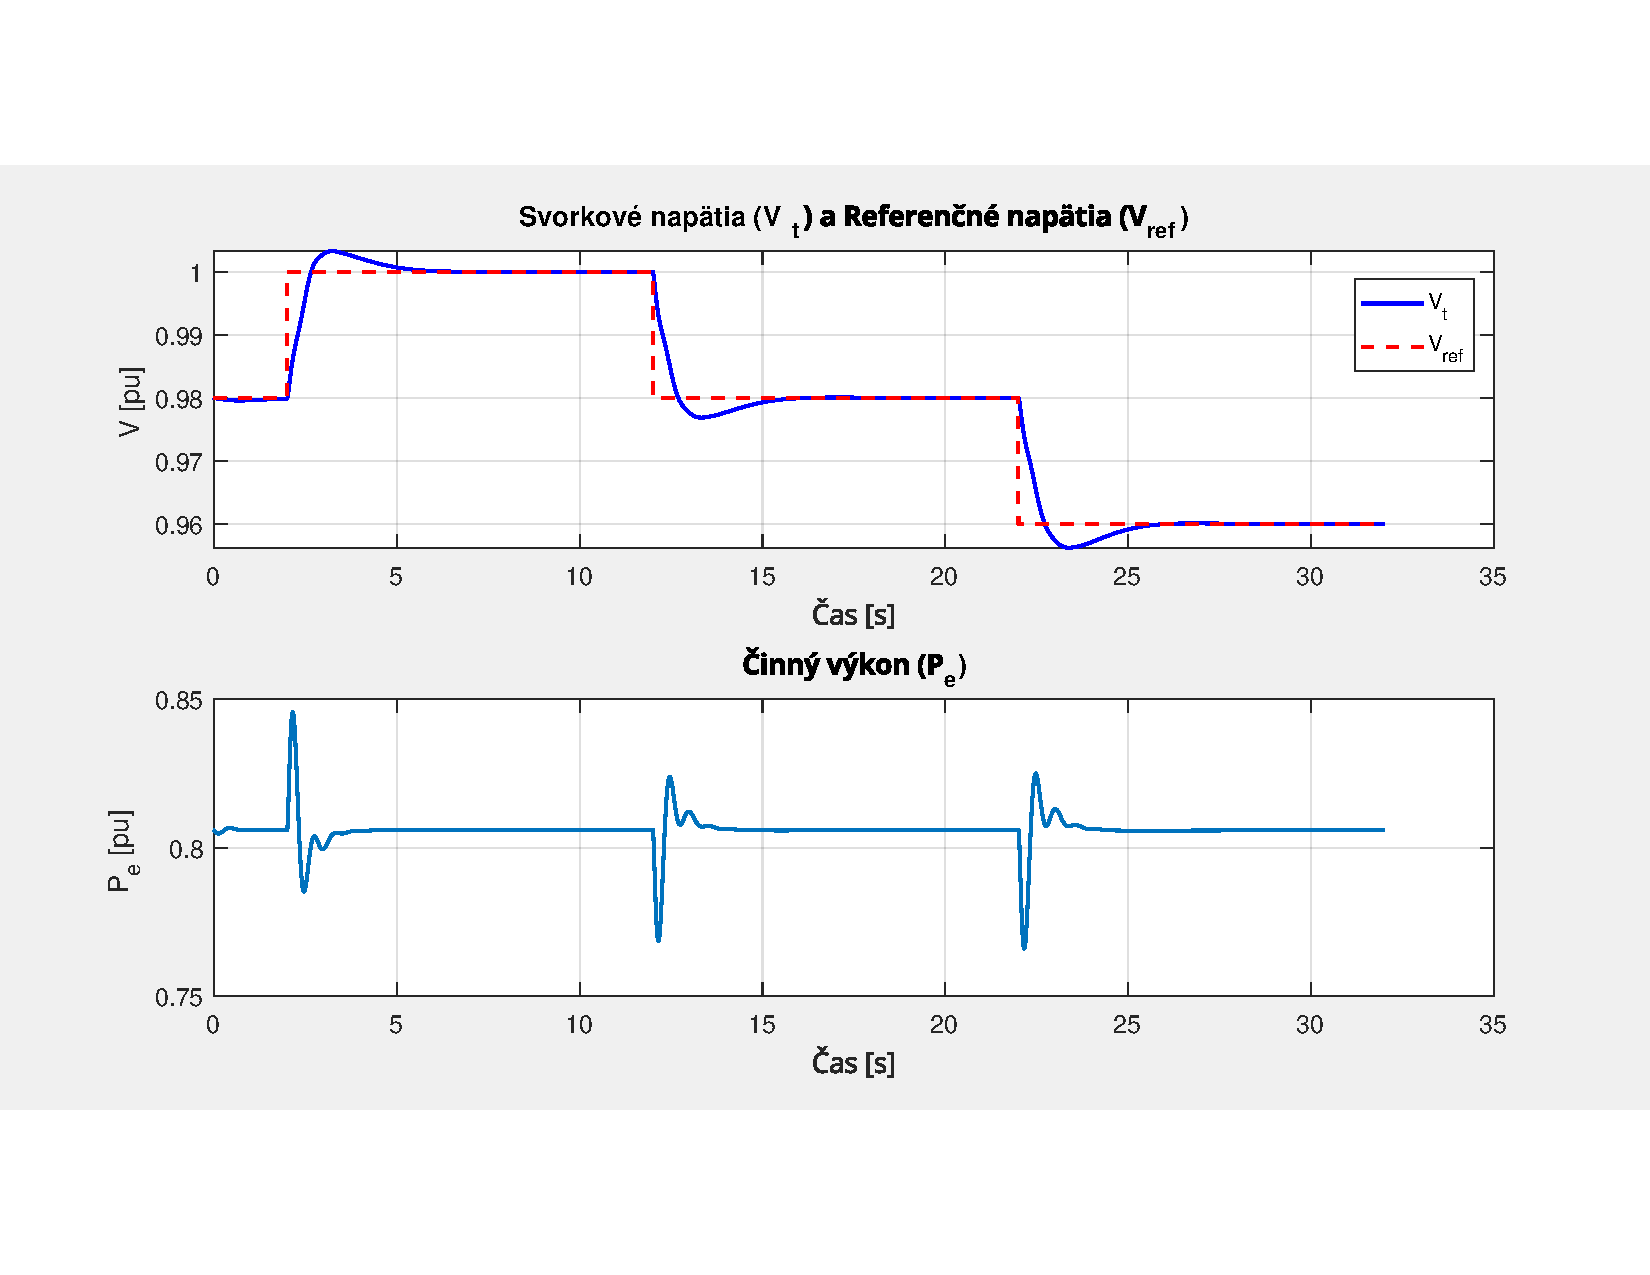
\includegraphics[width=1\textwidth, trim=1.5cm 3.2cm 2.2cm 3.5cm, clip]{img/Response_best4_Pe.pdf}
    \caption{Prechodová charakteristika svorkového napätia a činného výkonu synchrónneho generátora}
    \label{fig:prechodove_char}
\end{figure} 

Na obrázku \ref{fig:prechodove_char} sú zobrazené odozvy svorkového napätia a činného výkonu synchrónneho generátorana skokové zmeny referenčného napätia, ktoré je v obrázku znázornené červenou farbou. Ako je možné vidieť, pri skokovej zmene žiadaného napätia dochádza ku krátkodobému prekmitu svorkového napätia a kmitaniu činného výkonu. K rýchlejšiemu tlmeniu kmitania prispieva použitie stabilizátora PSS a ladenie parametrov regulátora turbíny, ktoré sú popísané v kapitole \ref{sec:optimalizacia}.

Pre tento konkrétny priebeh simulácie boli parametre PSS a regulátora turbíny nastavené na nasledujúce hodnoty, ktoré sú výsledkom optimalizácie: $T_1 = 0.3006 s$, $T_2 = 0.1131 s$, $K_{pe} = 0.8$, $K_p = 0.001$ a $K_i = 0.07$.

Pre vytvorenie frekvenčných charakteristík činného výkonu bol použitý ako referenčný signál napäria sinusový signál s amplitúdou $0.01 p.u.$ a frekvenciou v rozsahu od $0.1 Hz$ do $5.5 Hz$ s krokom $0.05 Hz$. Pre každný krok frekvencie bola vykonaná simulácia, z ktorej boli získané priebehy hodnoty činného výkonu. V týchto priebehoch boli následne nájdené hodnoty peakov s použitím funkcie \texttt{findpeaks} v MATLABe, z ktorých boli následné vykreslené frekvenčné charakteristiky činného výkonu. 

\begin{figure}[h]
    \centering
    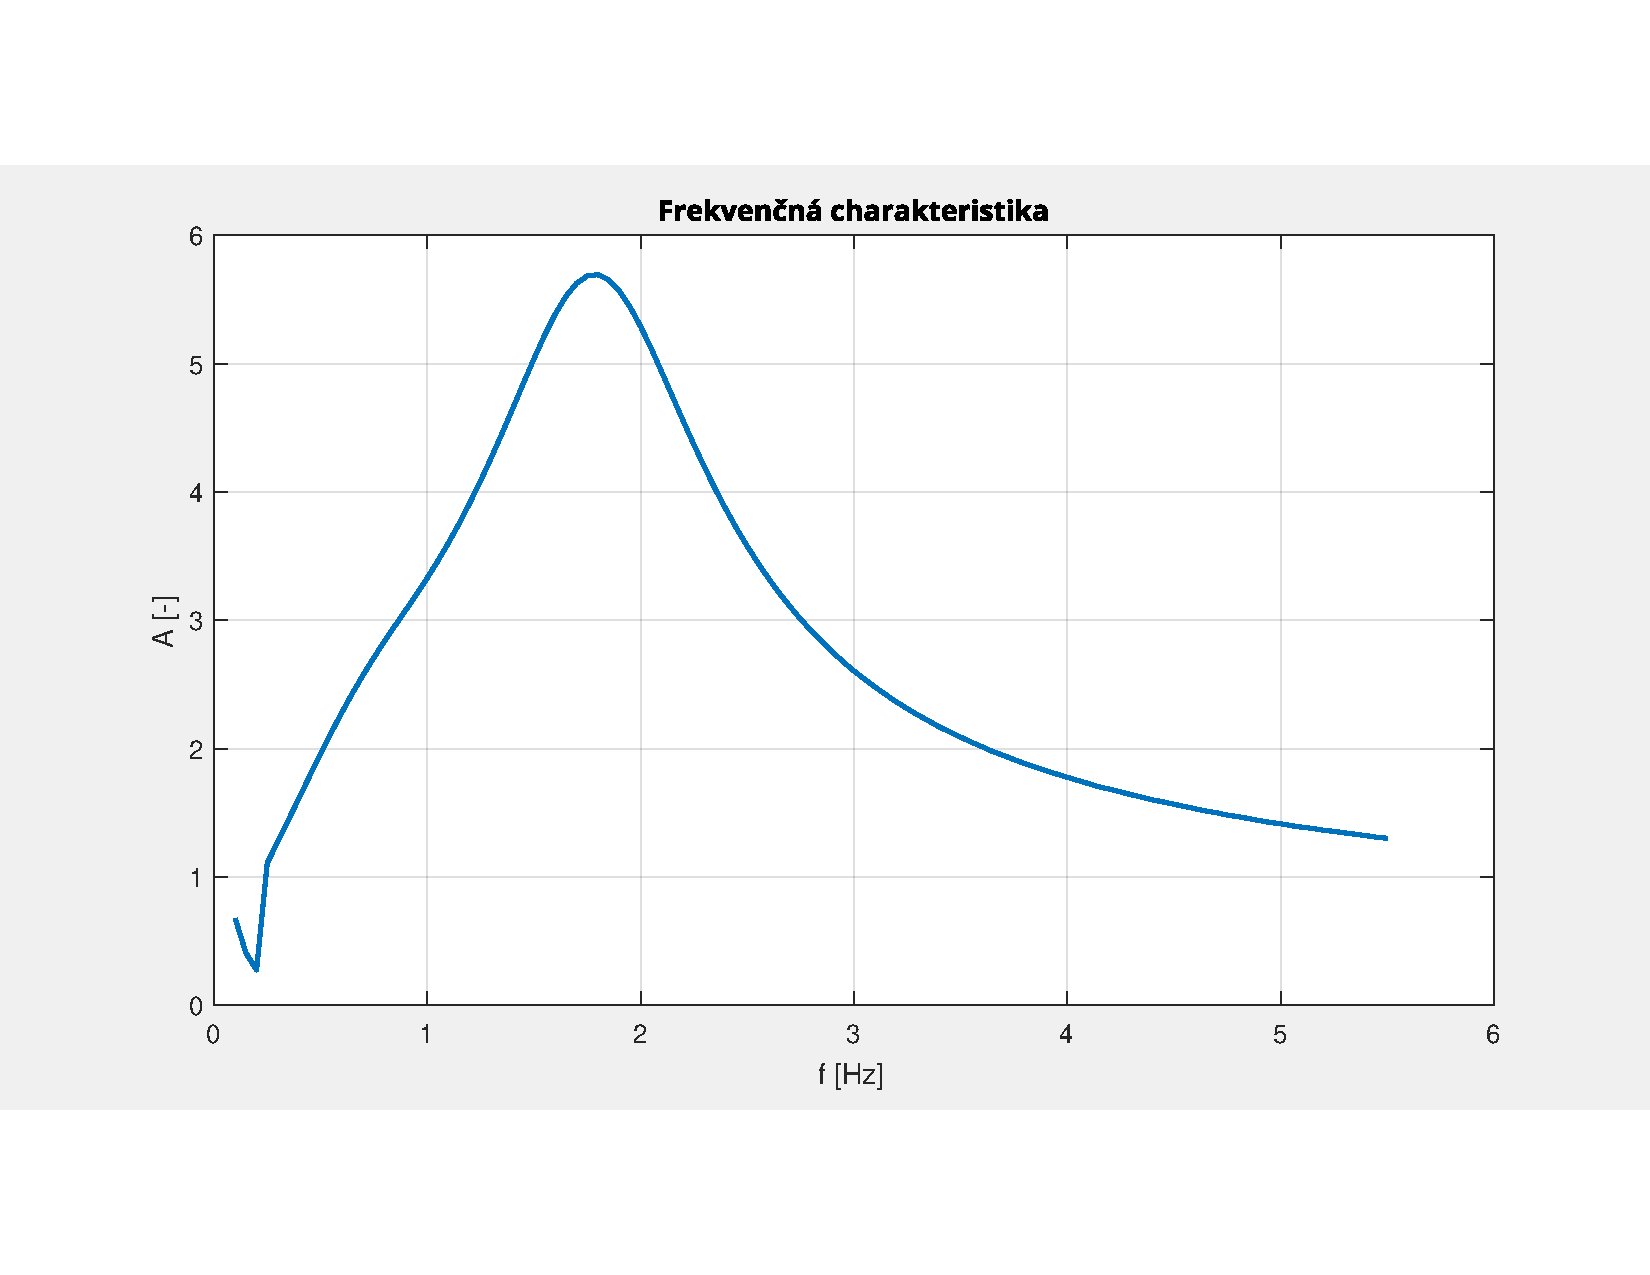
\includegraphics[width=0.8\textwidth, trim=1.5cm 3.2cm 2.2cm 3.2cm, clip]{img/Freq_char_4_Pe.pdf}
    \caption{Frekvenčná charakteristika činného výkonu $P_e$}
    \label{fig:freq_char}
\end{figure}

Na obrázku \ref{fig:freq_char} je zobrazená frekvenčná charakteristika činného výkonu $P_e$, ktorá bola vytvorená s nastavením parametrov PSS a regulátora turbíny, ktoré boli použité aj pre priebeh simulácie zobrazený na obrázku \ref{fig:prechodove_char}, a to $T_1 = 0.3006 s$, $T_2 = 0.1131 s$, $K_{pe} = 0.8$, $K_p = 0.001$ a $K_i = 0.07$. Z frekvenčnej charakteristiky je možné pozorovať, že najvyššia amplitúda, približne $5.7 p.u.$, je dosiahnutá pri frekvencii približne $1.8 Hz$.

Na tvar a amplitúdu frekvenčnej charakteristiky činného výkonu má vplyv nastavenie parametrov PSS a regulátora turbíny. Porovnanie vplyvu nastavenia je zobrazené v porovnaní priebehov v kapitole \ref{sec:optimalizacia}.